%%% Lecture 9

\section{More on Fibre Bundles and Fibrations}

\lecture[Some more fibre bundles/fibrations stuff. Prof. Schwede suggests that we take the categorical red pill. Shout-out to the category of compactly generated spaces (without definition). We introduce the compact-open topology.]{2021-11-15}

Prof. Schwede is back!

\begin{theorem}
Let $p:E\to B$ be a continuous map, with path-connected base.
\begin{numerate}
    \item If $p$ is a Hurewicz fibration, then any two fibers of $p$ are homotopy equivalent.
    \item If $p$ is a Serre fibration, then any two fibres which are CW-complexes are homotopy equivalent.
\end{numerate}
\end{theorem}

\begin{proof}
Let $b_0,b_1\in B$ be points, set $F_0=p^{-1}(b_0),F_1=p^{-1}(b_1)$.

Let $\omega:[0,1]\to B$ be a path from $b_0$ to $b_1$. Choose homotopies $H$ and $K$ as liftings in the followings diagrams:
\begin{center}
\begin{tikzcd}[column sep=large]
F_0\times 0 \arrow[r,"\incl"] \arrow[d,hook] & E \arrow[d,"p"] \\
F_0\times[0,1] \arrow[ur,dashed,"H"] \arrow[r,"\omega\circ\pr_2"] & B
\end{tikzcd}\qquad
\begin{tikzcd}[column sep=large]
F_1\times 0 \arrow[r,"\incl"] \arrow[d,hook] & E \arrow[d,"p"] \\
F_1\times[0,1] \arrow[ur,dashed,"K"] \arrow[r,"\bar\omega\circ\pr_2"] & B
\end{tikzcd}
\end{center}

where $\bar\omega(t)=\omega(1-t)$ is the inverse path.

We set $f=H(-,1):F_0\to F_1$ and $g=K(-,1):F_1\to F_0$.

Let $L:[0,1]\times[0,1]\to B$ be a homotopy, relative $\cb{0,1}$, from the concatenated path $\omega*\bar\omega$ to $\const_{b_0}$.
\[L(-,0)=\omega*\bar\omega,\]
\[L(-,1)=\const_{b_0}\]
\[L(0,t)=L(1,t)=b_0\]

Choose another lifting in the following diagram:

\begin{center}
    \begin{tikzcd}[column sep=huge]
    F_0\times((0\times I)\cup(I\times 0)\cup(1\times I)) \arrow[r] \arrow[d,hook] & E \arrow[d,"p"] \\

    F_0\times[0,1]\times[0,1] \arrow[ur,dashed,swap,"\bar L"] \arrow[r,swap,"L\circ\pr_{2,3}"] & B
    \end{tikzcd}
\end{center}
where the upper arrow is\alvaropls\ $(\const_{\incl}\,\cup\, H*(K\circ(f\times\id))\,\cup\,\const_{g\circ f})$.\smallskip

\begin{center}
    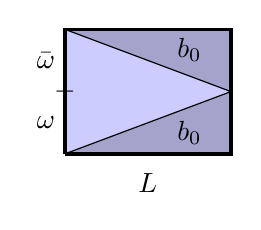
\begin{tikzpicture}[x=1.5em, y=1.5em, baseline=2.1em]
    \filldraw[very thick, fill=blue!20] (0,0)--(0,3)--(4,3)--(4,0)--(0,0);
    \draw (0,0)--(4,1.5)--(0,3);
    \filldraw[fill = black, opacity = 0.2] (0,0)--(4,1.5)--(0,3)--(4,3)--(4,0)--(0,0);
    \filldraw
    (0,.75) node[anchor=east]{$\omega$}
    (0,2.25) node[anchor=east]{$\bar\omega$}
    (0,1.5) node {$-$}
    (3,2.5) node {$b_0$}
    (3,0.5) node {$b_0$}
    (2,-0.7) node{$L$};
    \end{tikzpicture}
    \hspace{2cm}
    \(\displaystyle
    \begin{tikzcd}[column sep=huge]
    F_0\times
        
\begin{tikzpicture}[x=1em, y=1em, baseline=0.2em]
        \draw[very thick] (0,1)--(0,0)--(1,0)--(1,1);
        \end{tikzpicture}
    \arrow[r] \arrow[d,hook] & E \arrow[d,"p"] \\
    F_0\times
        
\begin{tikzpicture}[x=1em, y=1em, baseline=0.2em]
        \filldraw[very thick, fill=blue!20] (1,0)--(0,0)--(0,1)--(1,1)--(1,0);
        \end{tikzpicture}
    \arrow[ur,dashed,swap,"\bar L"] \arrow[r,swap,"L\circ\pr_{2,3}"] & B
    \end{tikzcd}\)
\end{center}

\vspace{-0.1cm}
Then we can set $G=\bar L(-,-,1):F_0\times[0,1]\to E$ to obtain a homotopy from $\incl:F_0\into E$ to $\incl\circ g\circ f:F_0\to E$.

Since $p\circ G=\const_{b_0}$, this homotopy $G$ takes place inside $F_0$. So $G$ can be seen as a homotopy from $\id_{F_0}$ to $g\circ f$. Reversing the roles of $b_0$ with $b_1$, $F_0$ with $F_1$ and $f$ with $g$ yields a homotopy from $\id_{F_1}$ to $f\circ g$.
\end{proof}

\unnumpar{Induced fibres bundles/fibrations}

We construct the pullback bundle\rightnote{This construction is also called base change sometimes. Or fiber product.}. Let $p:E\to B$ and $\beta:B'\to B$ be continuous maps. The pullback is \[E'=B'\times_B E=\cb{(b',e)\in B'\times E\mid \beta(b')=p(e)}\]
with subspace topology of the product topology.

\begin{center}
    \begin{tikzcd}
    &[-6ex] (b',e) \arrow[r,mapsto] & e \\[-4ex]
    (b',e) \arrow[d,mapsto] & B'\times_B E \arrow[d,dashed,"p'"] \arrow[r,dashed,"\beta'"] & E \arrow[d,"p"] \\
    
    b' & B' \arrow[r,"\beta"] & B
    \end{tikzcd}
\end{center}

This is a pullback in $\Top$ in the sense of category theory, i.e. the following universal property holds: for all spaces $A$ and continuous maps $\alpha:A\to B'$ and $\epsilon:A\to E$ such that $\beta\alpha=p\epsilon$, there is a unique continuous map $\delta:A\to B'\times_B E$ such that $\beta'\delta=\epsilon$ and $\alpha\delta=p'$, namely the map $\delta(a)=(\alpha(a),\epsilon(a))$.
\begin{center}
    \begin{tikzcd}
    A \arrow[dr,dashed,"\exists!\delta"] \arrow[drr,bend left,"\epsilon"] \arrow[ddr,bend right,"\alpha"] & & \\
     & B'\times_B E \arrow[d,"p'"] \arrow[r,"\beta'"] & E \arrow[d,"p"] \\
    
     & B' \arrow[r,"\beta"] & B
    \end{tikzcd}
\end{center}

\begin{example}[Restriction bundle]
Suppose $B'$ is a subspace of $B$ and $\beta:B'\to B$ the inclusion. Then we have
\[B'\times_B E\cong p^{-1}(B')\]
with homeomorphisms given by
\[(b',e)\mapsto e,\]
\[(p(e),e)\mapsfrom e.\]
\end{example}

\begin{example}[A pretty stupid one]
I lost the explanation, but take it as a little rebus:
\begin{center}
    \begin{tikzcd}
    B'\amalg B' \arrow[d] \arrow[r] & B' \arrow[d] \\
    *\amalg* \arrow[r] & *
    \end{tikzcd}
\end{center}
\end{example}
In general taking the constant map $\beta:B'\to B$ to a point $b\in B$ will yield as the pullback bundle the trivial bundle $B'\times p^{-1}(b)$.

\begin{theorem}
Let $p:E\to B$ and $\beta:B'\to B$ be continuous maps.
\begin{itemize}
    \item[(i)] If $p$ is a fibre bundle, then so is $p':B'\times_B E\to B'$.
    \item[(ii)] If $p$ is a Hurewicz fibration, then so is $p'$.
    \item[(iii)] If $p$ is a Serre fibration, then so is $p'$.
\end{itemize}
\end{theorem}

\begin{proof}\rightnote{\emph{\enquote{You take the blue pill — the story ends, you wake up in your bed and believe whatever you want to believe. You take the red pill — you stay in Wonderland, and I show you how deep the rabbit hole goes.}}}There's two reasonable proofs of the first fact, one direct, one categorical. The Professor seems to be suggesting a blue pill/red pill situation (with the categorical version being \emph{\enquote{much more transparent}} to him).

(i) Consider any point $a\in B'$. There is a open neighbourhood $U$ of $\beta(a)$ in $B$ and a local trivialization, i.e. a homeomorphism $\psi:p^{-1}(U)\to U\times F$ for one space $F$ (over $U$).

We argue that $p':B'\times_B E\to B'$ is trivializable over $V=\beta^{-1}(U)$ with the same fibre $F$.

The following are mutually inverse homeomorphisms:
\begin{align*}
    (p')^{-1}(V)&\xleftrightarrow{\ \cong\ }V\times F\\
    (b',e)&\ \,\mapsto\ (b',\psi_2(e))\\
    (b',\psi^{-1}(\beta(b'),f))&\ \,\mapsfrom\ (b',f).
\end{align*}

Categorical proof: the statement is an instance of the fact that \enquote{pullbacks are transitive}.

In any category $\Cc$, we consider a commutative diagram:
\begin{center}
    \begin{tikzcd}[column sep={8em,between origins}]
    B''\times_B E \arrow[d] \arrow[r] & B'\times_B E \arrow[d,"p'"] \arrow[r,"\beta'"] & E \arrow[d] \\
    
    B'' \arrow[r] & B' \arrow[r,"\beta"] & B
    \end{tikzcd}
\end{center}

If both squares are pullbacks, then the composite square is also a pullback. Symbolic notation:
\[B''\times_B E\cong B''\times_{B'}(B'\times_B E).\]

Hence, considering the same situation as in the direct proof, we have:
\[(p')^{-1}(V)=V\times_B E\cong V\times_{B'}(B'\times_B E)= V\times_U(U\times_B E)\cong V\times_U(U\times F)\cong V\times F.\]

(ii)+(iii) We show: whenever $p:E\to B$ has the HPL for some space $X$, then $p':B'\times_B E\to B'$ also has the HLP for $X$.

Consider a lifting square on the left:
\begin{center}
    \begin{tikzcd}[column sep=large,row sep=huge]
    X\times0 \arrow[d,hook] \arrow[r,"f"] & B'\times_B E \arrow[d,"p'" near end] \arrow[r,"\beta'"] & E \arrow[d,"p"] \\
    
    X\times[0,1] \arrow[ur,dashed,bend left=20,blue,"\bar K"] \arrow[urr,dashed,crossing over,red, "K" near start] \arrow[r,"H"'] & B' \arrow[r,"\beta"'] & B
    \end{tikzcd}
\end{center}

There is a homotopy $K:X\times[0,1]\to E$ so that $p\circ K=\beta\circ H$ and $K(-,0)=\beta'\circ f$.

The universal property of the pullback provides a unique continuous map
\[\bar K:X\times[0,1]\to B'\times_B E\]
such that $p'\circ \bar K=H$ and $\beta'\circ\bar K=K$.

The two continuous maps $f,\,\bar K(-,0):X\times0\to B'\times_B E$ compose in the same way with $p'$ and with $\beta'$. The uniqueness part of the universal property then forces $f=\bar K(-,0)$.
\end{proof}

\chapter{Mapping Spaces}

\section{Compact-open Topology}

Our aim: to define and study a specific topology on $Z^X=\cb{f:X\to Z\text{ continuous}}.$

We would like the "exponential law" to hold: the map
\begin{align*}
    Z^{X\times Y}&\to(Z^X)^Y\\
    (f:X\times Y\to Z)&\mapsto \cb{y\mapsto f(-,y)}
\end{align*}
should be a homeomorphism.

Unfortunately, it is not. At least not in general, but the good news is that it is whenever $Y$ is Hausdorff and $X$ locally compact.

\begin{remark}
There is a way to arrange the exponential law in complete generality: work in the full subcategory $CG$ of compactly generated spaces. Then $CG$ is a cartesian closed category, i.e. it has finite products and for all $X\in\operatorname{ob}(G)$
\[-\times X:CG\to CG\]
has a right adjoint, written $Z\mapsto Z^X$.

Watch out: the product in $CG$ is not always the usual product topology!

Some examples of classes of spaces in $CG$ are:
\begin{itemize}[label={-}]
    \item every locally compact Hausdorff space,
    \item every CW-complex,
    \item every manifold is in $CG$,
    \item the realization of every simplicial set,
    \item for two CW-complexes $X$ and $Y$, the product in $CG$, $X\times_{CG}Y$, is again a CW-complex.
    \item for all simplicial sets $A,B$, the canonical map:
    \[|A\times B|\to|A|\times_{CG}|B|\]
    is a homeomorphism.
\end{itemize}
\end{remark}

Enter: the compact-open topology. For spaces $X$ and $Z$, write $Z^X$ for the set of continuous maps $f:X\to Z$. Let $K$ be a compact subset of $X$ and let $O$ be an open subset of $Z$. Set:
\[W(K,O)=\cb{f\in Z^X:f(K)\subset O}\subset Z^X.\]

The \textbf{compact-open topology} on $Z^X$ is the topology generated by the sets $W(K,O)$ with $K\subset X$ compact and $O\subset Z$ open, i.e. these sets form a subbasis of the compact-open topology.

\begin{theorem}
Let $X$ be a compact space and $(Z,d)$ a metric space.
\begin{numerate}
\item There is a metric on $Z^X$, defined as:
\[d(g_1,g_2)=\sup_{x\in X}d(g_1(x),g_2(x)),\text{ for }g_1,g_2\in Z^X.\]
called the supremum metric.
\item The compact-open topology on $Z^X$ coincides with the metric topology of the supremum metric.
\end{numerate}
\end{theorem}

\begin{proof}
(1) Omitted (see \cite[Proposition A.13]{hatcher}).

(2) \enquote{$\subset$}: compact-open is metrically open.

It suffices to show that the generating sets $W(K,O)$ are metrically open. Fix $K\subset X$ compact, $O\subset Z$ open and $f\in W(K,O)$, i.e. $f(K)\subset O$. Then $C=Z\sm O$ is a closed subset of $Z$ and $f(x)\not\in C$ for all $x\in K$ (hence $d(f(x),C)>0$ for all $x\in K$). Since $K$ is compact, $\epsilon=\inf_{x\in K}d(f(x),C)>0$
is positive.
We claim that $B_{\sup}(f,\epsilon)\subset W(K,O)$.

Let $g\in Z^X$ be such that $d(f,g)<\epsilon$. Then $d(f(x),g(x))<\epsilon$ for all $x\in K$, hence:
\[d(f(x),g(x))\leq d(f(x),C),\]
so $g(x)\in O=Z\sm C$. Therefore $g(K)\subset O$, so $g\in W(K,O)$.

\enquote{$\supset$}: metrically open is compact-open.

Let $A\subset Z^X$ be open in the sup-topology, $f\in A$. We will construct finitely many compact sets $K_i$ in $X$ and open sets $O_i$ in $Z$ so that:
\[f\in W(K_1,O_1)\cap\dots\cap W(K_m,O_m)\subset A.\]

Since $A$ is open in the sup-topology, there is an $\epsilon>0$ so that $A$ contains the $\epsilon$-ball around $f$.

For $x\in X$ the set $f^{-1}(B(f(x),\epsilon/5))$ is an open neighbourhood of $x$ in $X$. Since $X$ is compact\rightnote{Note: compact spaces, meaning quasi-compact \textit{and} Hausdorff, are locally compact, but quasi-compact spaces may not be!}, this contains a compact neighbourhood $K_x$ of $x$. Since $X$ is compact, there are finitely many $x_1,\dots,x_m$ such that $X=K_{x_1}\cup\dots\cup K_{x_m}$.
Set $K_i:=K_{x_i}$ and $O_i:=$ open $\epsilon/5$-neighbourhood of $f(K_i)$ in $Z$.

\input{Pictures/Lec9Pic2}
As shown in the picture, for all $z,z'\in O_i$, we have $d(z,z')\leq 4\epsilon/5<\epsilon$ (to expand on this, observe we have $f(K_x) \subset B(f(x),\frac{\varepsilon}{5})\subseteq O_x := \frac{\varepsilon}{5}\text{-neighborhood of }f(K_x)$, hence both $z$ and $z'$ are at distance less or equal than $\frac{\varepsilon}{5}$ from two points of $f(K_x)$, and both these points are at distance less or equal than $\frac{\varepsilon}{5}$ from $f(x)$).

Suppose that $g\in W(K_1,O_1)\cap\dots\cap W(K_m,O_m)$. Then for all $x\in X$ there is $1\leq i\leq m$ with $x\in K_i$. Since $g\in W(K_i,O_i)$, we have $g(x)\in O_i$. We also have $x\in K_i=K_{x_i}$, so $d(f(x),f(x_i))\leq\epsilon/5$ so $f(x)\in O_i$. Hence $d(g(x),f(x))<\epsilon$. Since this holds for all $x\in X$, $d(f,g)<\epsilon$. So $W(K_1,O_1)\cap\dots\cap W(K_m,O_m)\subset B_{\sup}(f,\epsilon)\subset A$.
\end{proof}
